
%% IAENG_pub.tex 2010/08/30
%% It is based on the bare_jrnl.tex V1.3 2007/01/11 by Michael Shell
%% see http://www.michaelshell.org/
%% for current contact information.
%%
%% This is a skeleton file demonstrating the use of IAENGtran.cls
%% (requires IAENGtran.cls version 1.7 or later) with an IAENG journal/conference paper.
%%
%% Support sites:
%% http://www.michaelshell.org/tex
%% http://www.ctan.org/tex-archive/macros/latex/contrib/IEEEtran/

% *** Authors should verify (and, if needed, correct) their LaTeX system  ***
% *** with the testflow diagnostic prior to trusting their LaTeX platform ***
% *** with production work. IAENG's font choices can trigger bugs that do  ***
% *** not appear when using other class files.                            ***
% The testflow support page is at:
% http://www.michaelshell.org/tex/testflow/


%%*************************************************************************
%% Legal Notice:
%% This code is offered as-is without any warranty either expressed or
%% implied; without even the implied warranty of MERCHANTABILITY or
%% FITNESS FOR A PARTICULAR PURPOSE!
%% User assumes all risk.
%% In no event shall IAENG or any contributor to this code be liable for
%% any damages or losses, including, but not limited to, incidental,
%% consequential, or any other damages, resulting from the use or misuse
%% of any information contained here.
%%
%% All comments are the opinions of their respective authors and are not
%% necessarily endorsed by the IAENG.
%%
%% This work is distributed under the LaTeX Project Public License (LPPL)
%% ( http://www.latex-project.org/ ) version 1.3, and may be freely used,
%% distributed and modified. A copy of the LPPL, version 1.3, is included
%% in the base LaTeX documentation of all distributions of LaTeX released
%% 2003/12/01 or later.
%% Retain all contribution notices and credits.
%% ** Modified files should be clearly indicated as such, including  **
%% ** renaming them and changing author support contact information. **
%%
%%*************************************************************************

% Note that the a4paper option is mainly intended so that authors in
% countries using A4 can easily print to A4 and see how their papers will
% look in print - the typesetting of the document will not typically be
% affected with changes in paper size (but the bottom and side margins will).
% Use the testflow package mentioned above to verify correct handling of
% both paper sizes by the user's LaTeX system.
%
% Also note that the "draftcls" or "draftclsnofoot", not "draft", option
% should be used if it is desired that the figures are to be displayed in
% draft mode.
%
\documentclass[journal]{IAENGtran}
%
% If IAENGtran.cls has not been installed into the LaTeX system files,
% manually specify the path to it like:
% \documentclass[journal]{../sty/IAENGtran}





% Some very useful LaTeX packages include:
% (uncomment the ones you want to load)


% *** MISC UTILITY PACKAGES ***
%
%\usepackage{ifpdf}
% Heiko Oberdiek's ifpdf.sty is very useful if you need conditional
% compilation based on whether the output is pdf or dvi.
% usage:
% \ifpdf
%   % pdf code
% \else
%   % dvi code
% \fi
% The latest version of ifpdf.sty can be obtained from:
% http://www.ctan.org/tex-archive/macros/latex/contrib/oberdiek/
% Also, note that IAENGtran.cls V1.7 and later provides a builtin
% \ifCLASSINFOpdf conditional that works the same way.
% When switching from latex to pdflatex and vice-versa, the compiler may
% have to be run twice to clear warning/error messages.






% *** CITATION PACKAGES ***
%
%\usepackage{cite}
% cite.sty was written by Donald Arseneau
% V1.6 and later of IAENGtran pre-defines the format of the cite.sty package
% \cite{} output to follow that of IAENG. Loading the cite package will
% result in citation numbers being automatically sorted and properly
% "compressed/ranged". e.g., [1], [9], [2], [7], [5], [6] without using
% cite.sty will become [1], [2], [5]--[7], [9] using cite.sty. cite.sty's
% \cite will automatically add leading space, if needed. Use cite.sty's
% noadjust option (cite.sty V3.8 and later) if you want to turn this off.
% cite.sty is already installed on most LaTeX systems. Be sure and use
% version 4.0 (2003-05-27) and later if using hyperref.sty. cite.sty does
% not currently provide for hyperlinked citations.
% The latest version can be obtained at:
% http://www.ctan.org/tex-archive/macros/latex/contrib/cite/
% The documentation is contained in the cite.sty file itself.






% *** GRAPHICS RELATED PACKAGES ***
%
\ifCLASSINFOpdf
   \usepackage[pdftex]{graphicx}
  % declare the path(s) where your graphic files are
   \graphicspath{{figures/}}
  % and their extensions so you won't have to specify these with
  % every instance of \includegraphics
   \DeclareGraphicsExtensions{.pdf,.jpeg,.png}
\else
  % or other class option (dvipsone, dvipdf, if not using dvips). graphicx
  % will default to the driver specified in the system graphics.cfg if no
  % driver is specified.
   \usepackage[dvips]{graphicx}
  % declare the path(s) where your graphic files are
   \graphicspath{{figures/}}
  % and their extensions so you won't have to specify these with
  % every instance of \includegraphics
   \DeclareGraphicsExtensions{.eps}
\fi
% graphicx was written by David Carlisle and Sebastian Rahtz. It is
% required if you want graphics, photos, etc. graphicx.sty is already
% installed on most LaTeX systems. The latest version and documentation can
% be obtained at:
% http://www.ctan.org/tex-archive/macros/latex/required/graphics/
% Another good source of documentation is "Using Imported Graphics in
% LaTeX2e" by Keith Reckdahl which can be found as epslatex.ps or
% epslatex.pdf at: http://www.ctan.org/tex-archive/info/
%
% latex, and pdflatex in dvi mode, support graphics in encapsulated
% postscript (.eps) format. pdflatex in pdf mode supports graphics
% in .pdf, .jpeg, .png and .mps (metapost) formats. Users should ensure
% that all non-photo figures use a vector format (.eps, .pdf, .mps) and
% not a bitmapped formats (.jpeg, .png). IAENG frowns on bitmapped formats
% which can result in "jaggedy"/blurry rendering of lines and letters as
% well as large increases in file sizes.
%
% You can find documentation about the pdfTeX application at:
% http://www.tug.org/applications/pdftex



% *** MATH PACKAGES ***
%
\usepackage[cmex10]{amsmath}
% A popular package from the American Mathematical Society that provides
% many useful and powerful commands for dealing with mathematics. If using
% it, be sure to load this package with the cmex10 option to ensure that
% only type 1 fonts will utilized at all point sizes. Without this option,
% it is possible that some math symbols, particularly those within
% footnotes, will be rendered in bitmap form which will result in a
% document that can not be IAENG compliant!
%
% Also, note that the amsmath package sets \interdisplaylinepenalty to 10000
% thus preventing page breaks from occurring within multiline equations. Use:
%\interdisplaylinepenalty=2500
% after loading amsmath to restore such page breaks as IAENGtran.cls normally
% does. amsmath.sty is already installed on most LaTeX systems. The latest
% version and documentation can be obtained at:
% http://www.ctan.org/tex-archive/macros/latex/required/amslatex/math/





% *** SPECIALIZED LIST PACKAGES ***
%
%\usepackage{algorithmic}
% algorithmic.sty was written by Peter Williams and Rogerio Brito.
% This package provides an algorithmic environment for describing algorithms.
% You can use the algorithmic environment in-text or within a figure
% environment to provide for a floating algorithm. Do NOT use the algorithm
% floating environment provided by algorithm.sty (by the same authors) or
% algorithm2e.sty (by Christophe Fiorio) as IAENG does not use dedicated
% algorithm float types and packages that provide these will not provide
% correct IAENG style captions. The latest version and documentation of
% algorithmic.sty can be obtained at:
% http://www.ctan.org/tex-archive/macros/latex/contrib/algorithms/
% There is also a support site at:
% http://algorithms.berlios.de/index.html
% Also of interest may be the (relatively newer and more customizable)
% algorithmicx.sty package by Szasz Janos:
% http://www.ctan.org/tex-archive/macros/latex/contrib/algorithmicx/




% *** ALIGNMENT PACKAGES ***
%
%\usepackage{array}
% Frank Mittelbach's and David Carlisle's array.sty patches and improves
% the standard LaTeX2e array and tabular environments to provide better
% appearance and additional user controls. As the default LaTeX2e table
% generation code is lacking to the point of almost being broken with
% respect to the quality of the end results, all users are strongly
% advised to use an enhanced (at the very least that provided by array.sty)
% set of table tools. array.sty is already installed on most systems. The
% latest version and documentation can be obtained at:
% http://www.ctan.org/tex-archive/macros/latex/required/tools/


%\usepackage{mdwmath}
%\usepackage{mdwtab}
% Also highly recommended is Mark Wooding's extremely powerful MDW tools,
% especially mdwmath.sty and mdwtab.sty which are used to format equations
% and tables, respectively. The MDWtools set is already installed on most
% LaTeX systems. The lastest version and documentation is available at:
% http://www.ctan.org/tex-archive/macros/latex/contrib/mdwtools/


% IAENGtran contains the IAENGeqnarray family of commands that can be used to
% generate multiline equations as well as matrices, tables, etc., of high
% quality.


%\usepackage{eqparbox}
% Also of notable interest is Scott Pakin's eqparbox package for creating
% (automatically sized) equal width boxes - aka "natural width parboxes".
% Available at:
% http://www.ctan.org/tex-archive/macros/latex/contrib/eqparbox/

\usepackage{tabularx}
\usepackage{multirow}
\usepackage{booktabs}

\newcolumntype{Y}{>{\centering\arraybackslash}X}





% *** SUBFIGURE PACKAGES ***
%\usepackage[tight,footnotesize]{subfigure}
% subfigure.sty was written by Steven Douglas Cochran. This package makes it
% easy to put subfigures in your figures. e.g., "Figure 1a and 1b". For IAENG
% work, it is a good idea to load it with the tight package option to reduce
% the amount of white space around the subfigures. subfigure.sty is already
% installed on most LaTeX systems. The latest version and documentation can
% be obtained at:
% http://www.ctan.org/tex-archive/obsolete/macros/latex/contrib/subfigure/
% subfigure.sty has been superceeded by subfig.sty.



%\usepackage[caption=false]{caption}
%\usepackage[font=footnotesize]{subfig}
% subfig.sty, also written by Steven Douglas Cochran, is the modern
% replacement for subfigure.sty. However, subfig.sty requires and
% automatically loads Axel Sommerfeldt's caption.sty which will override
% IAENGtran.cls handling of captions and this will result in nonIAENG style
% figure/table captions. To prevent this problem, be sure and preload
% caption.sty with its "caption=false" package option. This is will preserve
% IAENGtran.cls handing of captions. Version 1.3 (2005/06/28) and later
% (recommended due to many improvements over 1.2) of subfig.sty supports
% the caption=false option directly:
%\usepackage[caption=false,font=footnotesize]{subfig}
%
% The latest version and documentation can be obtained at:
% http://www.ctan.org/tex-archive/macros/latex/contrib/subfig/
% The latest version and documentation of caption.sty can be obtained at:
% http://www.ctan.org/tex-archive/macros/latex/contrib/caption/




% *** FLOAT PACKAGES ***
%
%\usepackage{fixltx2e}
% fixltx2e, the successor to the earlier fix2col.sty, was written by
% Frank Mittelbach and David Carlisle. This package corrects a few problems
% in the LaTeX2e kernel, the most notable of which is that in current
% LaTeX2e releases, the ordering of single and double column floats is not
% guaranteed to be preserved. Thus, an unpatched LaTeX2e can allow a
% single column figure to be placed prior to an earlier double column
% figure. The latest version and documentation can be found at:
% http://www.ctan.org/tex-archive/macros/latex/base/



%\usepackage{stfloats}
% stfloats.sty was written by Sigitas Tolusis. This package gives LaTeX2e
% the ability to do double column floats at the bottom of the page as well
% as the top. (e.g., "\begin{figure*}[!b]" is not normally possible in
% LaTeX2e). It also provides a command:
%\fnbelowfloat
% to enable the placement of footnotes below bottom floats (the standard
% LaTeX2e kernel puts them above bottom floats). This is an invasive package
% which rewrites many portions of the LaTeX2e float routines. It may not work
% with other packages that modify the LaTeX2e float routines. The latest
% version and documentation can be obtained at:
% http://www.ctan.org/tex-archive/macros/latex/contrib/sttools/
% Documentation is contained in the stfloats.sty comments as well as in the
% presfull.pdf file. Do not use the stfloats baselinefloat ability as IAENG
% does not allow \baselineskip to stretch. Authors submitting work to the
% IAENG should note that IAENG rarely uses double column equations and
% that authors should try to avoid such use. Do not be tempted to use the
% cuted.sty or midfloat.sty packages (also by Sigitas Tolusis) as IAENG does
% not format its papers in such ways.


%\ifCLASSOPTIONcaptionsoff
%  \usepackage[nomarkers]{endfloat}
% \let\MYoriglatexcaption\caption
% \renewcommand{\caption}[2][\relax]{\MYoriglatexcaption[#2]{#2}}
%\fi
% endfloat.sty was written by James Darrell McCauley and Jeff Goldberg.
% This package may be useful when used in conjunction with IAENGtran.cls'
% captionsoff option. Some IAENG journals/societies require that submissions
% have lists of figures/tables at the end of the paper and that
% figures/tables without any captions are placed on a page by themselves at
% the end of the document. If needed, the draftcls IAENGtran class option or
% \CLASSINPUTbaselinestretch interface can be used to increase the line
% spacing as well. Be sure and use the nomarkers option of endfloat to
% prevent endfloat from "marking" where the figures would have been placed
% in the text. The two hack lines of code above are a slight modification of
% that suggested by in the endfloat docs (section 8.3.1) to ensure that
% the full captions always appear in the list of figures/tables - even if
% the user used the short optional argument of \caption[]{}.
% IAENG papers do not typically make use of \caption[]'s optional argument,
% so this should not be an issue. A similar trick can be used to disable
% captions of packages such as subfig.sty that lack options to turn off
% the subcaptions:
% For subfig.sty:
% \let\MYorigsubfloat\subfloat
% \renewcommand{\subfloat}[2][\relax]{\MYorigsubfloat[]{#2}}
% For subfigure.sty:
% \let\MYorigsubfigure\subfigure
% \renewcommand{\subfigure}[2][\relax]{\MYorigsubfigure[]{#2}}
% However, the above trick will not work if both optional arguments of
% the \subfloat/subfig command are used. Furthermore, there needs to be a
% description of each subfigure *somewhere* and endfloat does not add
% subfigure captions to its list of figures. Thus, the best approach is to
% avoid the use of subfigure captions (many IAENG journals avoid them anyway)
% and instead reference/explain all the subfigures within the main caption.
% The latest version of endfloat.sty and its documentation can obtained at:
% http://www.ctan.org/tex-archive/macros/latex/contrib/endfloat/
%
% The IAENGtran \ifCLASSOPTIONcaptionsoff conditional can also be used
% later in the document, say, to conditionally put the References on a
% page by themselves.





% *** PDF, URL AND HYPERLINK PACKAGES ***
%
\usepackage{url}
% url.sty was written by Donald Arseneau. It provides better support for
% handling and breaking URLs. url.sty is already installed on most LaTeX
% systems. The latest version can be obtained at:
% http://www.ctan.org/tex-archive/macros/latex/contrib/misc/
% Read the url.sty source comments for usage information. Basically,
% \url{my_url_here}.





% *** Do not adjust lengths that control margins, column widths, etc. ***
% *** Do not use packages that alter fonts (such as pslatex).         ***
% There should be no need to do such things with IAENGtran.cls V1.6 and later.
% (Unless specifically asked to do so by the journal or conference you plan
% to submit to, of course. )


% correct bad hyphenation here
% \hyphenation{op-tical net-works semi-conduc-tor}

\usepackage{algorithm}
\usepackage{algpseudocode}

\begin{document}
%
% paper title
% can use linebreaks \\ within to get better formatting as desired
\title{Implementation of Inverse Perspective Mapping Using ROS 2 for Object Position Estimation \\ on a Humanoid Soccer Robot}
%
%
% author names and IAENG memberships
% note positions of commas and nonbreaking spaces ( ~ ) LaTeX will not break
% a structure at a ~ so this keeps an author's name from being broken across
% two lines.
% use \thanks{} to gain access to the first footnote area
% a separate \thanks must be used for each paragraph as LaTeX2e's \thanks
% was not built to handle multiple paragraphs
%

\author{Faa'iz~Haikal~Hilmi,
        Rully~Soelaiman,~\IAENGmembership{Member,~IAENG}% <-this % stops a space
}% <-this % stops a space


% note the % following the last \IAENGmembership and also \thanks -
% these prevent an unwanted space from occurring between the last author name
% and the end of the author line. i.e., if you had this:
%
% \author{....lastname \thanks{...} \thanks{...} }
%                     ^------------^------------^----Do not want these spaces!
%
% a space would be appended to the last name and could cause every name on that
% line to be shifted left slightly. This is one of those "LaTeX things". For
% instance, "\textbf{A} \textbf{B}" will typeset as "A B" not "AB". To get
% "AB" then you have to do: "\textbf{A}\textbf{B}"
% \thanks is no different in this regard, so shield the last } of each \thanks
% that ends a line with a % and do not let a space in before the next \thanks.
% Spaces after \IAENGmembership other than the last one are OK (and needed) as
% you are supposed to have spaces between the names. For what it is worth,
% this is a minor point as most people would not even notice if the said evil
% space somehow managed to creep in.



% The paper headers
%\markboth{}%
%{Shell \MakeLowercase{\textit{et al.}}:}
% The only time the second header will appear is for the odd numbered pages
% after the title page when using the twoside option.
%
% *** Note that you probably will NOT want to include the author's ***
% *** name in the headers of peer review papers.                   ***
% You can use \ifCLASSOPTIONpeerreview for conditional compilation here if
% you desire.




% If you want to put a publisher's ID mark on the page you can do it like
% this:
%\IAENGpubid{0000--0000/00\$00.00~\copyright~2007 IAENG}
% Remember, if you use this you must call \IAENGpubidadjcol in the second
% column for its text to clear the IAENGpubid mark.



% use for special paper notices
%\IAENGspecialpapernotice{(Invited Paper)}




% make the title area
\maketitle

\pagestyle{empty}
\thispagestyle{empty}


\begin{abstract}
%\boldmath
Accurate vision-based distance estimation is a critical component of perception systems 
for humanoid soccer robots. Inverse Perspective Mapping (IPM) provides a geometric approach 
to estimate object positions from monocular camera images without additional distance sensors, 
which are prohibited in humanoid robot soccer competitions such as RoboCup. In practice, 
because of camera extrinsic parameters changing continuously caused by walking motion and 
head movements, IPM is challenging to implement reliably. 

This paper presents the implementation of IPM to estimate object distance on a humanoid soccer robot using ROS 2, 
a widely used robotics framework that enables modular and real-time data exchange between multiple robot subsystems, 
including sensors and processing modules. The proposed system integrates 
object detection outputs, camera intrinsic parameters, and real-time kinematic transformation 
obtained from the robot model. Evaluations under static and walking conditions 
show that the system produces stable object position estimation with an average error within 
X centimeters in static scenarios and X centimeters during walking.
\end{abstract}
% IAENGtran.cls defaults to using nonbold math in the Abstract.
% This preserves the distinction between vectors and scalars. However,
% if the journal you are submitting to favors bold math in the abstract,
% then you can use LaTeX's standard command \boldmath at the very start
% of the abstract to achieve this. Many IAENG journals frown on math
% in the abstract anyway.

% Note that keywords are not normally used for peerreview papers.
\begin{IAENGkeywords}
IPM, Humanoid Robot, ROS 2
\end{IAENGkeywords}






% For peer review papers, you can put extra information on the cover
% page as needed:
% \ifCLASSOPTIONpeerreview
% \begin{center} \bfseries EDICS Category: 3-BBND \end{center}
% \fi
%
% For peerreview papers, this IAENGtran command inserts a page break and
% creates the second title. It will be ignored for other modes.
\IAENGpeerreviewmaketitle



\section{Introduction} \label{sec:intro}
% The very first letter is a 2 line initial drop letter followed
% by the rest of the first word in caps.
%
% form to use if the first word consists of a single letter:
% \IAENGPARstart{A}{demo} file is ....
%
% form to use if you need the single drop letter followed by
% normal text (unknown if ever used by IAENG):
% \IAENGPARstart{A}{}demo file is ....
%
% Some journals put the first two words in caps:
% \IAENGPARstart{T}{his demo} file is ....
%
% Here we have the typical use of a "T" for an initial drop letter
% and "HIS" in caps to complete the first word.
\IAENGPARstart{H}{umanoid} robots are designed to operate in environments intended
for humans with body structures and capabilities similar to humans \cite{Kajita2014}.
Research on humanoid robots has increased significantly across various domains \cite{Siciliano2010}.
One benchmark for evaluating these advancements is competitive soccer for evaluating autonomous systems 
in real-time perception and dynamic stability \cite{RoboCupHumanoidLeague2025}. The RoboCup initiative sets a long-range goal: by 2050, 
a team of fully autonomous humanoid robots shall win a soccer game against the winner of the most 
recent FIFA World Cup \cite{RobocupFederation2026}.

To encourage human-like perception, the RoboCup Humanoid League competition rules restrict the use of non-human sensors. 
Distance sensors such as LiDAR and depth cameras are prohibited, forcing teams to rely primarily on 
vision sensors, inertial sensors, and joint encoders. Consequently, accurate distance estimation from a 
single camera remains a critical and challenging problem \cite{RoboCupHumanoidLeague2025}. Humanoid soccer robot must estimate 
the positions of objects such as the ball, goalposts, and field features to perform navigation 
and make decisions \cite{SatyaWidodo2012}.

Several approaches have been proposed for estimating object distance using visual data. Monocular Depth Estimation uses
deep learning approach to predict depth directly from a single image \cite{Zhang2025}. Although
it produces stable accuracy, this approach is computationally expensive and highly dependent on training
data, making it difficult to deploy on humanoid robots with limited computational resources \cite{Wofk2019}.
Stereo vision is another alternative that estimates depth from two cameras, but requires precise calibration
and is sensitive to lighting and texture variations, which reduces reliability in dynamic environments \cite{Kok2019}.

Inverse Perspective Mapping (IPM) offers a a lightweight geometric solution that estimates
objects positions by projecting image points by assuming that objects of interests lie on a planar surface, \cite{Li2024}.
IPM has been widely used in autonomus driving systems, where the camera pose is relatively fixed \cite{Bertozzi1998}. 
However, implementing IPM to humanoid robots is more challenging because the camera pose change continuously due
to body posture changes \cite{Dias2024}.

This paper presents the implementation of an IPM-based object position estimation system on a 
humanoid soccer robot developed by the ICHIRO ITS team. The objective of this work is to demonstrate 
how IPM can be integrated with real-time kinematic transformations in ROS 2 to estimate object positions 
under both static and dynamic conditions.

The remainder of this paper is organized as follows. Section II presents the overall system description, 
including the humanoid robot platform and the software framework used in this work. 
Section III introduces the theoretical background underlying the proposed approach, 
covering kinematic modeling and inverse perspective mapping principles. 
Section IV describes the implementation methodology of the system. 
Section V presents the experimental evaluation and results. 
Finally, Section VI concludes the paper and discusses future work.

\section{System Description} \label{sec:system_desc}

This section describes the humanoid robot platform and software framework used 
in this research, providing the system context in which the proposed approach is implemented.

\subsection{ICHIRO ITS}
The system is implemented on humanoid soccer robots developed by the ICHIRO ITS
team from Institut Teknologi Sepuluh Nopember. The team participates in humanoid
soccer competitions such as RoboCup, contributing to research and development
of humanoid robotics.

\begin{figure*}[t] % [t] places it at the top of the page
\centering
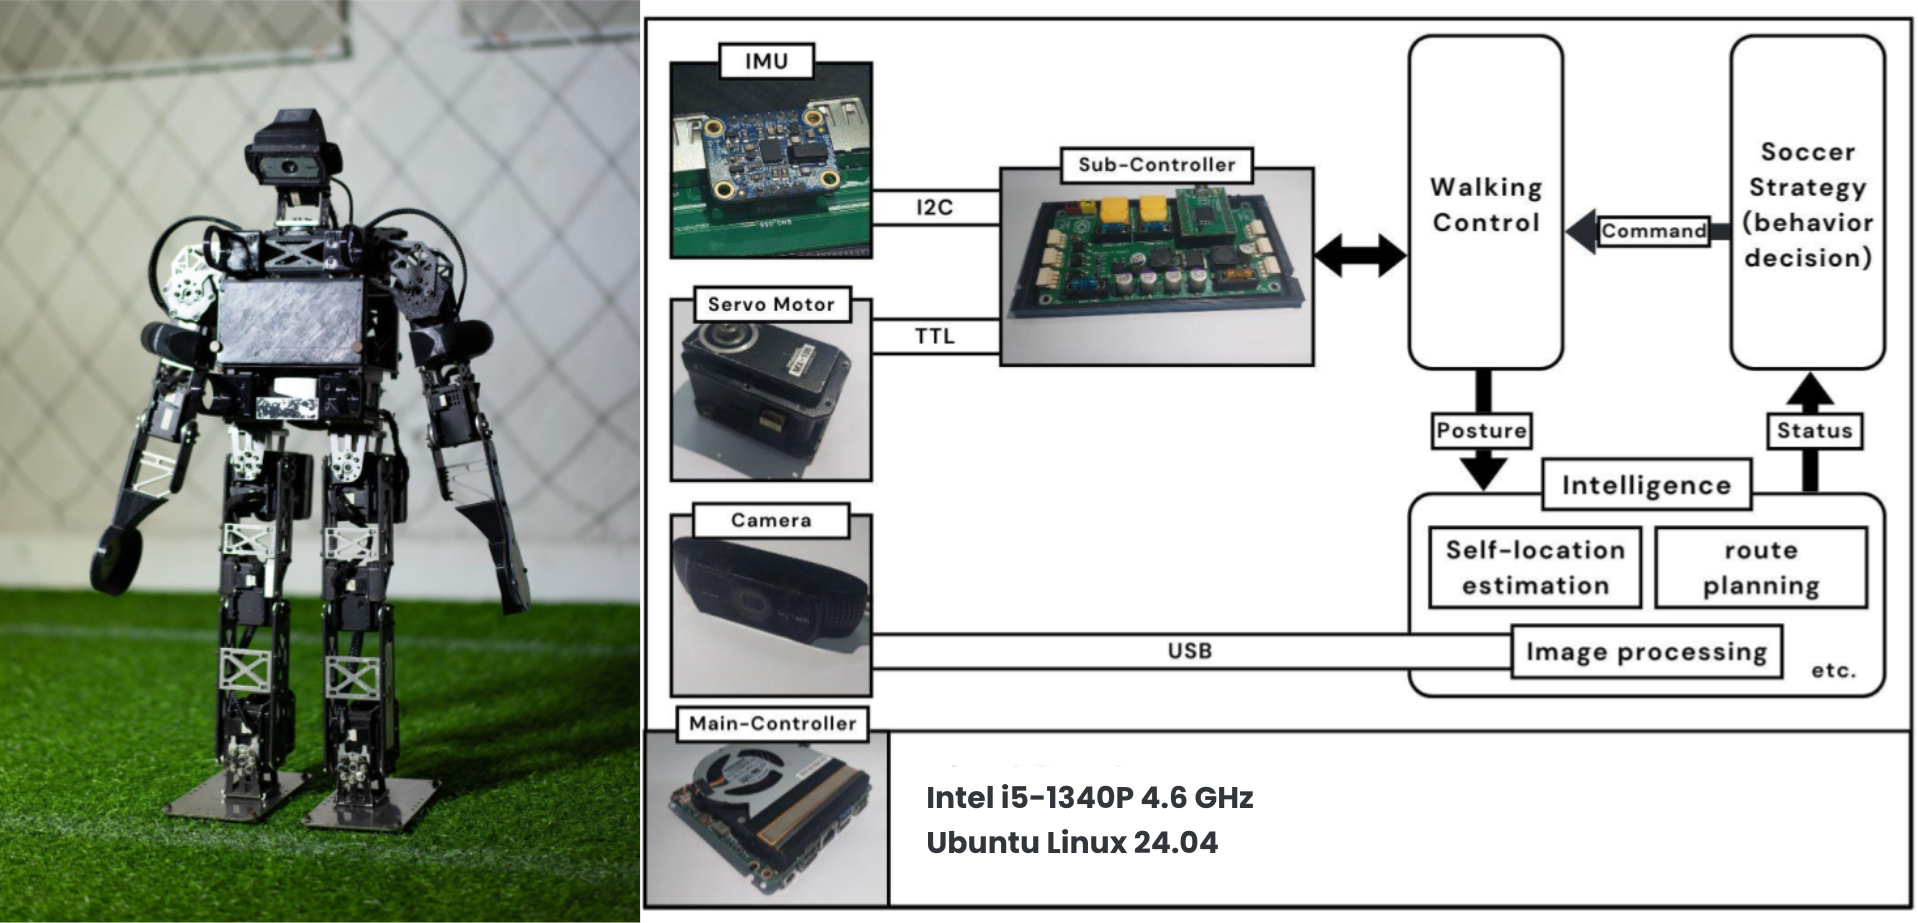
\includegraphics[width=\textwidth]{Ichiro Architecture.png}
\caption{ICHIRO ITS humanoid robot platform used in this research.}
\label{fig:ichiro}
\end{figure*}

The robot is classified as a kid-size humanoid, equipped with 20 Degrees of Freedom (DOF)
driven by servo actuators. A monocular RGB camera (Logitech C930e) is mounted on the robot's
head and serves as the primary sensor for perception. Additional sensors include joint
encoders for all actuated joints and an Inertial Measurement Unit (IMU) that provides
orientation information. The robot runs on an Intel NUC i5 mini PC, while a custom control
module (CM) board is responsible for low-level sensor acquisition and actuator interfacing.
An overview of the robot platform is shown in Figure ~\ref{fig:ichiro}.

\subsection{Robot Operating System 2}
The robot's software is built using the Robot Operating System 2 (ROS 2) 
Jazzy Jalisco, which provides a modular, multi-process architecture. 
The system utilizes the Data Distribution Service (DDS) middleware to 
ensure robust inter-process communication with configurable Quality of Service 
(QoS) policies. The ROS 2 framework facilitates a publisher-subscriber 
model that allows independent nodes to share information through standardized 
topics \cite{Macenski2022}.

In this research, the IPM implementation leverages existing software 
modules that publish: a Deep Neural Network (DNN) node for publishing 
detected objects as bounding boxes, a joint state publisher for real-time 
servo encoder values, and an IMU node for orientation feedback. These 
synchronized data streams provide the necessary inputs for the IPM deprojection 
algorithm, allowing the system to accurately correlate visual features in 
image space with the robot's physical configuration in the real world.

\subsection{Universal Robot Definition Format}

Universal Robot Definition Format (URDF) is an XML-based format used to 
modelize robot's physical structure. This format is widely supported by 
the robotics ecosystem, including ROS 2, and enables the construction of a 
complete transformation tree. This tree transformations is constructed using
the ROS 2 \texttt{tf2} library, which can be broadcasted by a publisher node, 
allowing other nodes to consume synchronized pose data for real-time calculations.

The URDF for the ICHIRO ITS robot incorporates the 20 DOF servo actuators 
along with a dedicated \texttt{camera\_frame}. This frame follows the 
standard ROS vision axis convention where the $Z$-axis points forward 
along the optical axis, the $Y$-axis points downward, and the $X$-axis 
points to the right \cite{NVIDIA2026}. Additionally, the model 
defines the \texttt{left\_foot\_frame} and \texttt{right\_foot\_frame}, 
which are utilized to dynamically compute the \texttt{base\_footprint}. 
This virtual frame serves as the primary ground-level reference for 
the \texttt{camera\_frame} in the IPM calculation, ensuring that visual 
deprojections are correctly referenced to the playing surface.

\section{Theoretical Background} \label{sec:theories}

This section presents the theoretical foundations required for the 
proposed approach, including camera projection models, kinematic transformations, 
ground plane assumption, and the IPM formulation.

\subsection{Pinhole Camera Model}

The pinhole camera model describes the relation of three-dimensional
world point and two dimensional image plane as shown in Equation \ref{eq:pinhole}.

\begin{equation} \label{eq:pinhole}
\begin{split}
\begin{pmatrix} x \\ y \\ 1 \end{pmatrix} &= 
\begin{bmatrix}
f_{x} & 0 & p_{x} & 0 \\
0 & f_{y} & p_{y} & 0 \\
0 & 0 & 1     & 0 
\end{bmatrix}
\begin{bmatrix}
R & t \\
0 & 1 \\
\end{bmatrix}
\begin{pmatrix} X \\ Y \\ Z \\ 1 \end{pmatrix} \\
&= K \begin{bmatrix} R & t \\ 0 & 1 \end{bmatrix}
\begin{pmatrix} X \\ Y \\ Z \\ 1 \end{pmatrix}
\end{split}
\end{equation}
where:
\begin{itemize}
    \item $(x, y)$: Coordinates of the projected point on the 2D image plane.
    \item $(X, Y, Z)$: Coordinates of the point in the 3D world coordinate system.
    \item $K$: The camera intrinsic matrix, parameters unique to specific camera hardware,  
               including the focal length $(f_x, f_y)$ and the principal point coordinates $(p_x, p_y)$.
    \item $R$: The camera rotation matrix $(3 \times 3)$, representing the orientation 
               of the camera in the world frame.
    \item $t$: The camera translation vector $(3 \times 1)$, representing the position 
               of the camera origin in the world frame.
\end{itemize}
This formulation follows the standard pinhole camera model widely used in computer
vision \cite{Hartley2003,Szeliski2011}.

\subsection{Kinematics Tree}
A kinematic tree represents the hierarchical relationship between rigid 
bodies (links) connected by joints. In this structure, each node corresponds 
to a specific coordinate frame, while the edges define the rigid transformations 
between parent and child frames. This mathematical representation allows the pose 
of any link or sensor within the tree to be computed relative to a global or local 
reference frame through the use of chained homogeneous transformations \cite{Craig1986,Siciliano2010}.

A rigid body transformation between two frames is represented using 
a $4 \times 4$ homogeneous transformation matrix as shown in Equation \ref{eq:transformation_matrix}.
\begin{equation} \label{eq:transformation_matrix}
\mathbf{T}_{a}^{b} = 
\begin{bmatrix}
\mathbf{R}_{a}^{b} & \mathbf{t}_{a}^{b} \\
\mathbf{0}^{T} & 1
\end{bmatrix}
\end{equation}
where $\mathbf{R}_{a}^{b}$ is a $3 \times 3$ rotation matrix and 
$\mathbf{t}_{a}^{b}$ is a $3 \times 1$ translation vector from frame 
$a$ to frame $b$. Using homogeneous transformation matrix, a point $P_a$ expressed 
in coordinate frame $a$ is transformed into frame $b$ as shown in 
Equation \ref{eq:transformation_equation}.
\begin{equation} \label{eq:transformation_equation}
\begin{bmatrix} P_b \\ 1 \end{bmatrix} = \mathbf{T}_{a}^{b} \begin{bmatrix} P_a \\ 1 \end{bmatrix}
\end{equation}
This representation is commonly used in robotics to model body structures and 
to compute forward kinematics \cite{Kajita2014}.

\subsection{Ground Plane Assumption}
Inverse Perspective Mapping relies on the assumption that objects of interest lie on a planar surface \cite{Mark2024}. 
In humanoid soccer, this assumption is valid for objects such as the ball, goalposts, and field markings, 
as the playing field is flat \cite{RoboCupHumanoidLeague2025}.

By constraining points to lie on a plane, we can recover the depth Zc along the optical axis
by defining a plane in the camera frame Pc using plane equation as shown in Equation \ref{eq:plane_camera}

\begin{equation} \label{eq:plane_camera}
n_c \cdot P_c + d = 0
\end{equation}
where $n_c = [n_x, n_y, n_z]^T$ is the plane normal in the camera frame and $d$ 
is the perpendicular distance from the camera origin to the plane \cite{Stewart2012}.

The normal $n_c$ can be derived by transforming the fixed ground normal from the \texttt{base\_footprint} 
frame to the \texttt{camera\_frame}. Since the IPM algorithm assumes that all objects of interest 
lie on a flat surface, the ground normal in the base frame is fixed as $n_b = [0, 0, 1]^T$.
By applying the rotation matrix $R_{b}^{c}$, we can express this 
normal in the camera's coordinate system as shown in Equation \ref{eq:plane_camera_wrt_base}

\begin{equation} \label{eq:plane_camera_wrt_base}
n_c = R_{b}^{c} \cdot n_b = \begin{bmatrix} r_{13} \\ r_{23} \\ r_{33} \end{bmatrix}
\end{equation}
where $r_{13}, r_{23}, r_{33}$ are elements of the third column of the rotation matrix $R_{b}^{c}$.

\subsection{Inverse Perspective Mapping}
Inverse Perspective Mapping (IPM) aims to recover the three-dimensional 
position of an image point under the assumption that it lies on a known 
planar surface, typically the ground. Given the camera intrinsic parameters 
and the camera pose relative to the ground, the depth of a projected image 
point can be analytically recovered \cite{Bertozzi1998,Park2023}.

The pixel $(x, y)$ in image plane can be converted to three-dimensional coordinate in 
camera frame $Pc = [X_c, Y_c, Z_c]$ using the inversion of pinhole camera model
mentioned in Equation \ref{eq:pinhole}, which:

\begin{equation} \label{eq:coordinate_camera} 
\begin{bmatrix} X_c \ Y_c \end{bmatrix} = Z_c 
\begin{bmatrix} \frac{x - p_x}{f_x} \\ \frac{y - p_y}{f_y} \end{bmatrix} = Z_c 
\begin{bmatrix} u \ v \end{bmatrix} 
\end{equation}
where $(u, v)$ are normalized image coordinates.

By substituting $P_c = [u Z_c, v Z_c, Z_c]^T$ into Equation \ref{eq:plane_camera}, with 
the distance $d$ from the plane in the \texttt{camera\_frame} equal to 
the camera translation $T_z$ along the vertical axis relative to the base frame.
Therefore, $Z_c$ can be calculated as shown in Equation \ref{eq:zc}.

\begin{equation} \label{eq:zc}
Z_c = \frac{-T_z}{n_x u + n_y v + n_z}
\end{equation}

Once $P_c$ is fully determined, the estimated position relative to the robot $P_w$ 
is obtained by transforming $P_c$ into the \texttt{base\_footprint} frame:

\begin{equation}
\begin{bmatrix} P_w \\ 1 \end{bmatrix} = \mathbf{T}_{c}^{b} \begin{bmatrix} P_c \\ 1 \end{bmatrix}
\end{equation}
where $\mathbf{T}_{c}^{b}$ is the $4 \times 4$ homogeneous transformation matrix. 
Notice that, the system rejects any results where $Z_c \leq 0$ or is undefined (NaN), 
as these indicate points behind the camera or parallel to the optical axis.

\section{Methodology}

This section describes the implementation of the proposed system on a humanoid soccer robot. 
The methodology focuses on practical aspects, including camera calibration, robot kinematic frame construction, 
and the integration of the IPM module for object distance estimation.

\subsection{Camera Calibration}
The objective of camera calibration is to obtain the intrinsic parameters ($K$)
required for the projection calculation between the three-dimensional world and two-dimensional
image plane as mentioned in Equation \ref{eq:pinhole}. In this paper, we utilized a Logitech C930e camera that was mounted
on the robot's head.

The calibration was conducted using standard $8 \times 6$ checkerboard with known 
square dimensions. We captured approximately 15 images of the checkerboard from
various distances and angles as shown in Figure \ref{fig:camera_calib}.

\begin{figure}[!h]
\centering
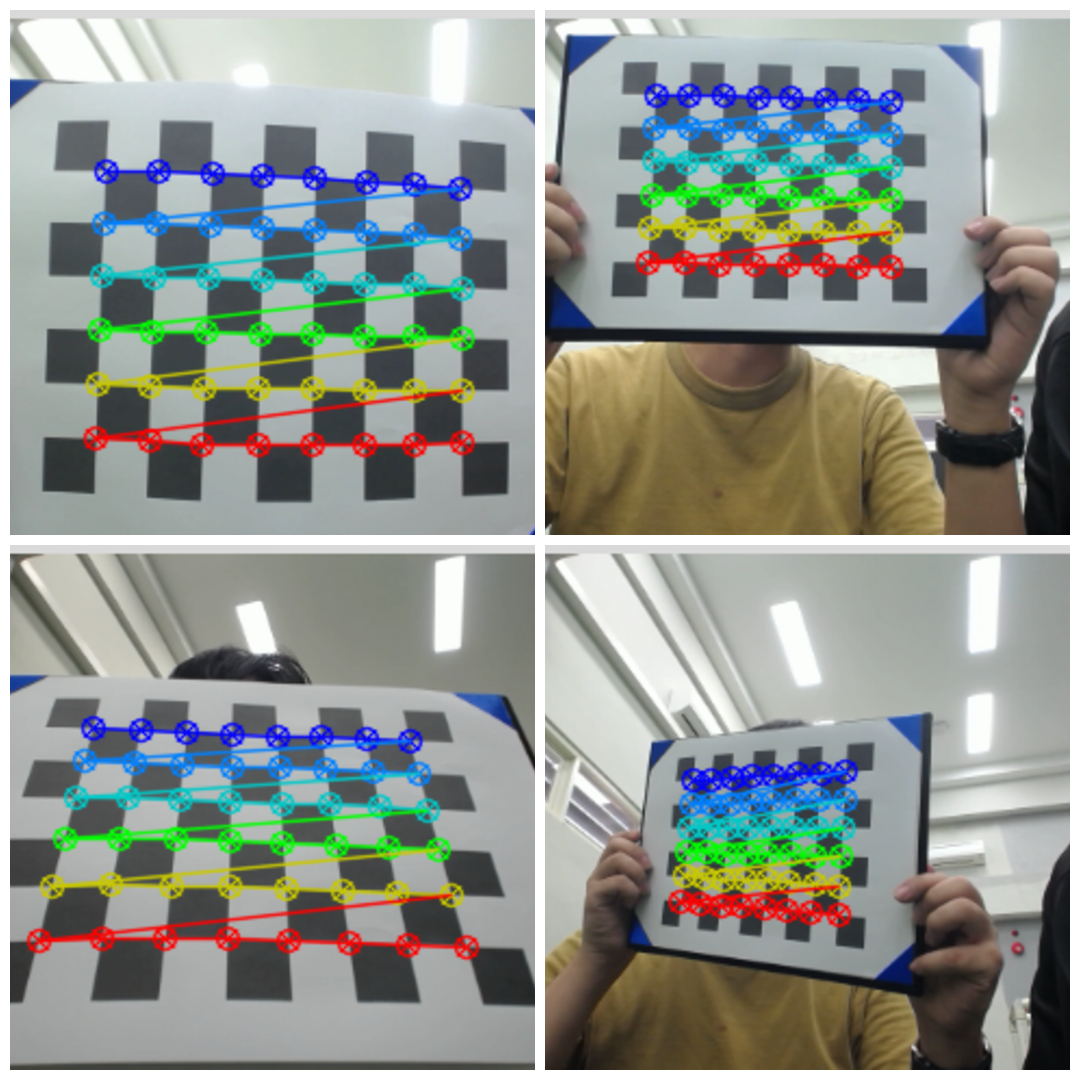
\includegraphics[width=3in,height=2.5in]{camera-calibration.png}
\caption{Visualization of detected checkerboard corners used for camera calibration.}
\label{fig:camera_calib}
\end{figure}

These images were then processed using OpenCV
calibration library to estimate the focal length $(f_x, f_y)$ and principal point 
coordinates $(p_x, p_y)$. While the calibration script also calculates lens distortion coefficients, the
radial and tangensial distortion values for the Logitech C930e were found to be
sufficiently small to be neglected.

\subsection{Robot Frames Package}
In this research, we implemented a dedicated ROS 2 package, \texttt{robot\_frames}, 
which loads the URDF model and broadcasts kinematic transformations using the \texttt{tf2} library. 
By consuming live joint encoder and IMU data, the package provides real-time kinematic transformations
that reflect the robot's physical state in the real world.

In addition, the package computes the \texttt{base\_footprint}, a virtual frame that serves as the 
reference frame for IPM calculations. This frame is calculated dynamically using information from 
the \texttt{right\_foot\_frame} and \texttt{left\_foot\_frame}. Since the robot is always in contact 
with the ground, the $Z$-height of the \texttt{base\_footprint} is set to match the supporting foot 
(i.e., the foot currently in contact with the ground). Meanwhile, the $X$ and $Y$ coordinates are 
defined as the midpoint between both feet.

\begin{algorithm}[!h]
\caption{Robot Frames Package}
\label{alg:robot_frames}
\footnotesize
\begin{algorithmic}[1]
\Require URDF path $(f)$
\Ensure TF frames $(\mathcal{T})$

\State $R \gets \text{ParseURDF}(f)$
\State $J \gets \text{ExtractJoints}(R)$

\While{running}
    \State $q \gets \text{ReadJointEncoders}()$
    \State $(r,p,\psi) \gets \text{ReadIMU}()$
    \State $(x,y) \gets \text{ReadOdometry}()$

    \State $\text{UpdateState}(q, r,p,\psi, x,y)$
    \State $\mathcal{T} \gets \emptyset$

    \ForAll{$j \in J$}
        \State $F \gets \text{ComputeTransform}(j)$
        \If{$j = \text{"body\_joint"}$}
            \State $F \gets \text{ApplyIMU}(F, r,p,\psi, x,y)$
        \EndIf
        \State $\mathcal{T} \gets \mathcal{T} \cup \{F\}$
    \EndFor

    \State $B \gets \text{ComputeBaseFootprint}()$
    \State $\mathcal{T} \gets \mathcal{T} \cup \{B\}$

    \State $\text{BroadcastTF}(\mathcal{T})$
\EndWhile

\end{algorithmic}
\end{algorithm}

\subsection{IPM Package}

We implemented another dedicated ROS~2 package, \texttt{ipm}, to perform distance estimation using 
the Inverse Perspective Mapping (IPM) algorithm. This package subscribes to object bounding boxes 
produced by a Deep Neural Network (DNN) detection module and kinematic transformations provided by 
the \texttt{robot\_frames} package. In addition, it loads a JSON configuration file containing the 
camera intrinsic parameters ($K$) obtained from the calibration process.

For each detected object, a representative image pixel $(x, y)$ is selected to approximate the 
object's contact point with the ground. For objects such as other robots or goalposts, the 
bottom-center of the bounding box is selected. For objects such as the ball or field markers, 
the center of the bounding box is used.

Note that for certain objects, such as the ball, the selected pixel may not correspond to direct 
ground contact. This discrepancy is handled by introducing a height offset ($h$), which effectively 
treats the ground plane as being elevated by that amount. Since the physical dimensions of the ball 
are known, the height offset $h$ corresponds to its radius. Consequently, the depth recovery 
equation derived in the Section \ref{sec:theories} is modified as follows:

\begin{equation} \label{eq:zc_final}
Z_c = \frac{T_z - h}{r_{13}u + r_{23}v + r_{33}}
\end{equation}

The remaining steps of the IPM algorithm follow the procedure described in 
Section \ref{sec:theories}.

\begin{algorithm}[!h]
\caption{IPM Package}
\label{alg:ipm}
\footnotesize
\begin{algorithmic}[1]
\Require TF Frames ($\mathcal{T}$)
\Ensure Projected Object Positions ($\mathcal{P}$)

\State $K \gets \text{LoadCameraIntrinsics}()$
\State $(f_x, f_y, c_x, c_y) \gets \text{ExtractIntrinsics}(K)$

\While{receiving detections}
    \State $\mathcal{O} \gets \text{ReadDetections}()$
    \State $\mathcal{P} \gets \emptyset$

    \ForAll{$o \in \mathcal{O}$}
        \State $u \gets (o.left + o.right)/2$
        \If{$o.\text{label} \in \{\text{"robot"}, \text{"goalpost"}\}$}
            \State $v \gets o.bottom$
        \Else
            \State $v \gets (o.top + o.bottom)/2$
        \EndIf

        \State $x \gets (u - c_x)/f_x$
        \State $y \gets (v - c_y)/f_y$

        \State $T \gets \text{LookupTransform}(\mathcal{T}, \text{camera} \rightarrow \text{base\_footprint})$
        \State $R \gets \text{RotationMatrix}(T)$
        \State $t \gets \text{TranslationVector}(T)$

        \State $h \gets 0$
        \If{$o.\text{label} = \text{ball}$}
            \State $h \gets \text{ball radius}$
        \EndIf

        \State $Z_c \gets \dfrac{t_z - h}{R_{13}x + R_{23}y + R_{33}}$
        \If{$Z_c \leq 0$}
            \State \textbf{continue}
        \EndIf

        \State $X_c \gets Z_c \cdot x$
        \State $Y_c \gets Z_c \cdot y$
        \State $P_c \gets (X_c, Y_c, Z_c)$

        \State $P_w \gets R \cdot P_c + t$

        \State $\mathcal{P} \gets \mathcal{P} \cup \{P_w\}$

    \EndFor

    \State $\text{Publish}(\mathcal{P})$
\EndWhile

\end{algorithmic}
\end{algorithm}

\section{Evaluation}

This section evaluates the performance of the proposed IPM-based distance 
estimation under static and dynamic conditions. Both evaluations are 
conducted using the same object configuration and identical initial 
robot position to ensure consistency. The static evaluation measures 
the intrinsic accuracy of IPM when the robot remains stationary, 
while the dynamic evaluation analyzes system behavior during walking 
and considers the influence of odometry when expressing results in 
global coordinates.

\subsection{Experimental Setup}

All experiments are conducted on a flat RoboCup soccer field ($6 \times 9$ m).
The robot is initialized at the same global position for both 
static and dynamic evaluations, namely the kickoff position 
$P(450.0, 300.0)$ at the center of the field.

A fixed set of objects is placed at known global coordinates 
and remains unchanged throughout all trials. 
Each object is assigned a symbolic notation for concise reference 
in subsequent tables and equations.

\begin{table}[h]
\centering
\caption{Fixed object configuration used in all experiments}
\label{tab:object_setup}
\begin{tabular}{c c c}
\hline
Symbol & Object & Global Position $(X_i, Y_i)$ [cm] \\
\hline
$O_1$ & Soccer Ball & $(550.0, 350.0)$ \\
$O_2$ & Opponent Robot & $(650.0, 200.0)$ \\
$O_3$ & Penalty Marker & $(750.0, 300.0)$ \\
$O_4$ & L-Intersection & $(800.0, 450.0)$ \\
$O_5$ & T-Intersection & $(900.0, 460.0)$ \\
$O_6$ & Left Goalpost & $(900.0, 170.0)$ \\
\hline
\end{tabular}
\end{table}

The global coordinates $(X_i, Y_i)$ are determined using field geometry 
and manual measurement to ensure repeatability. These positions remain 
constant for both static and dynamic experiments. A visualization of the 
experimental cpnfiguration is shown in Fig.~\ref{fig:experiment_setup}, while the actual experimental setup 
is presented in Fig.~\ref{fig:real_setup}.

\begin{figure}[!h]
\centering
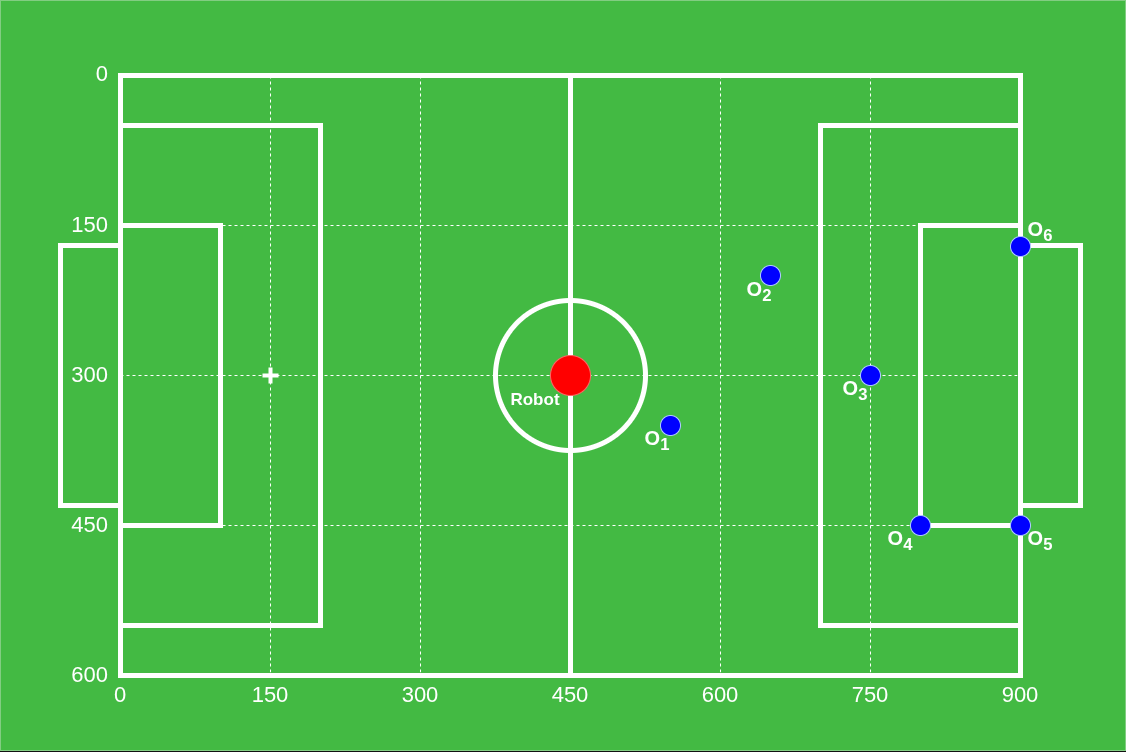
\includegraphics[width=0.5\textwidth]{Experiment Setup.png} 
\caption{Experimental setup showing the kickoff position of the robot 
and the fixed global positions of objects $O_1$–$O_6$ on the field.}
\label{fig:experiment_setup}
\end{figure}

\begin{figure}[!h]
\centering
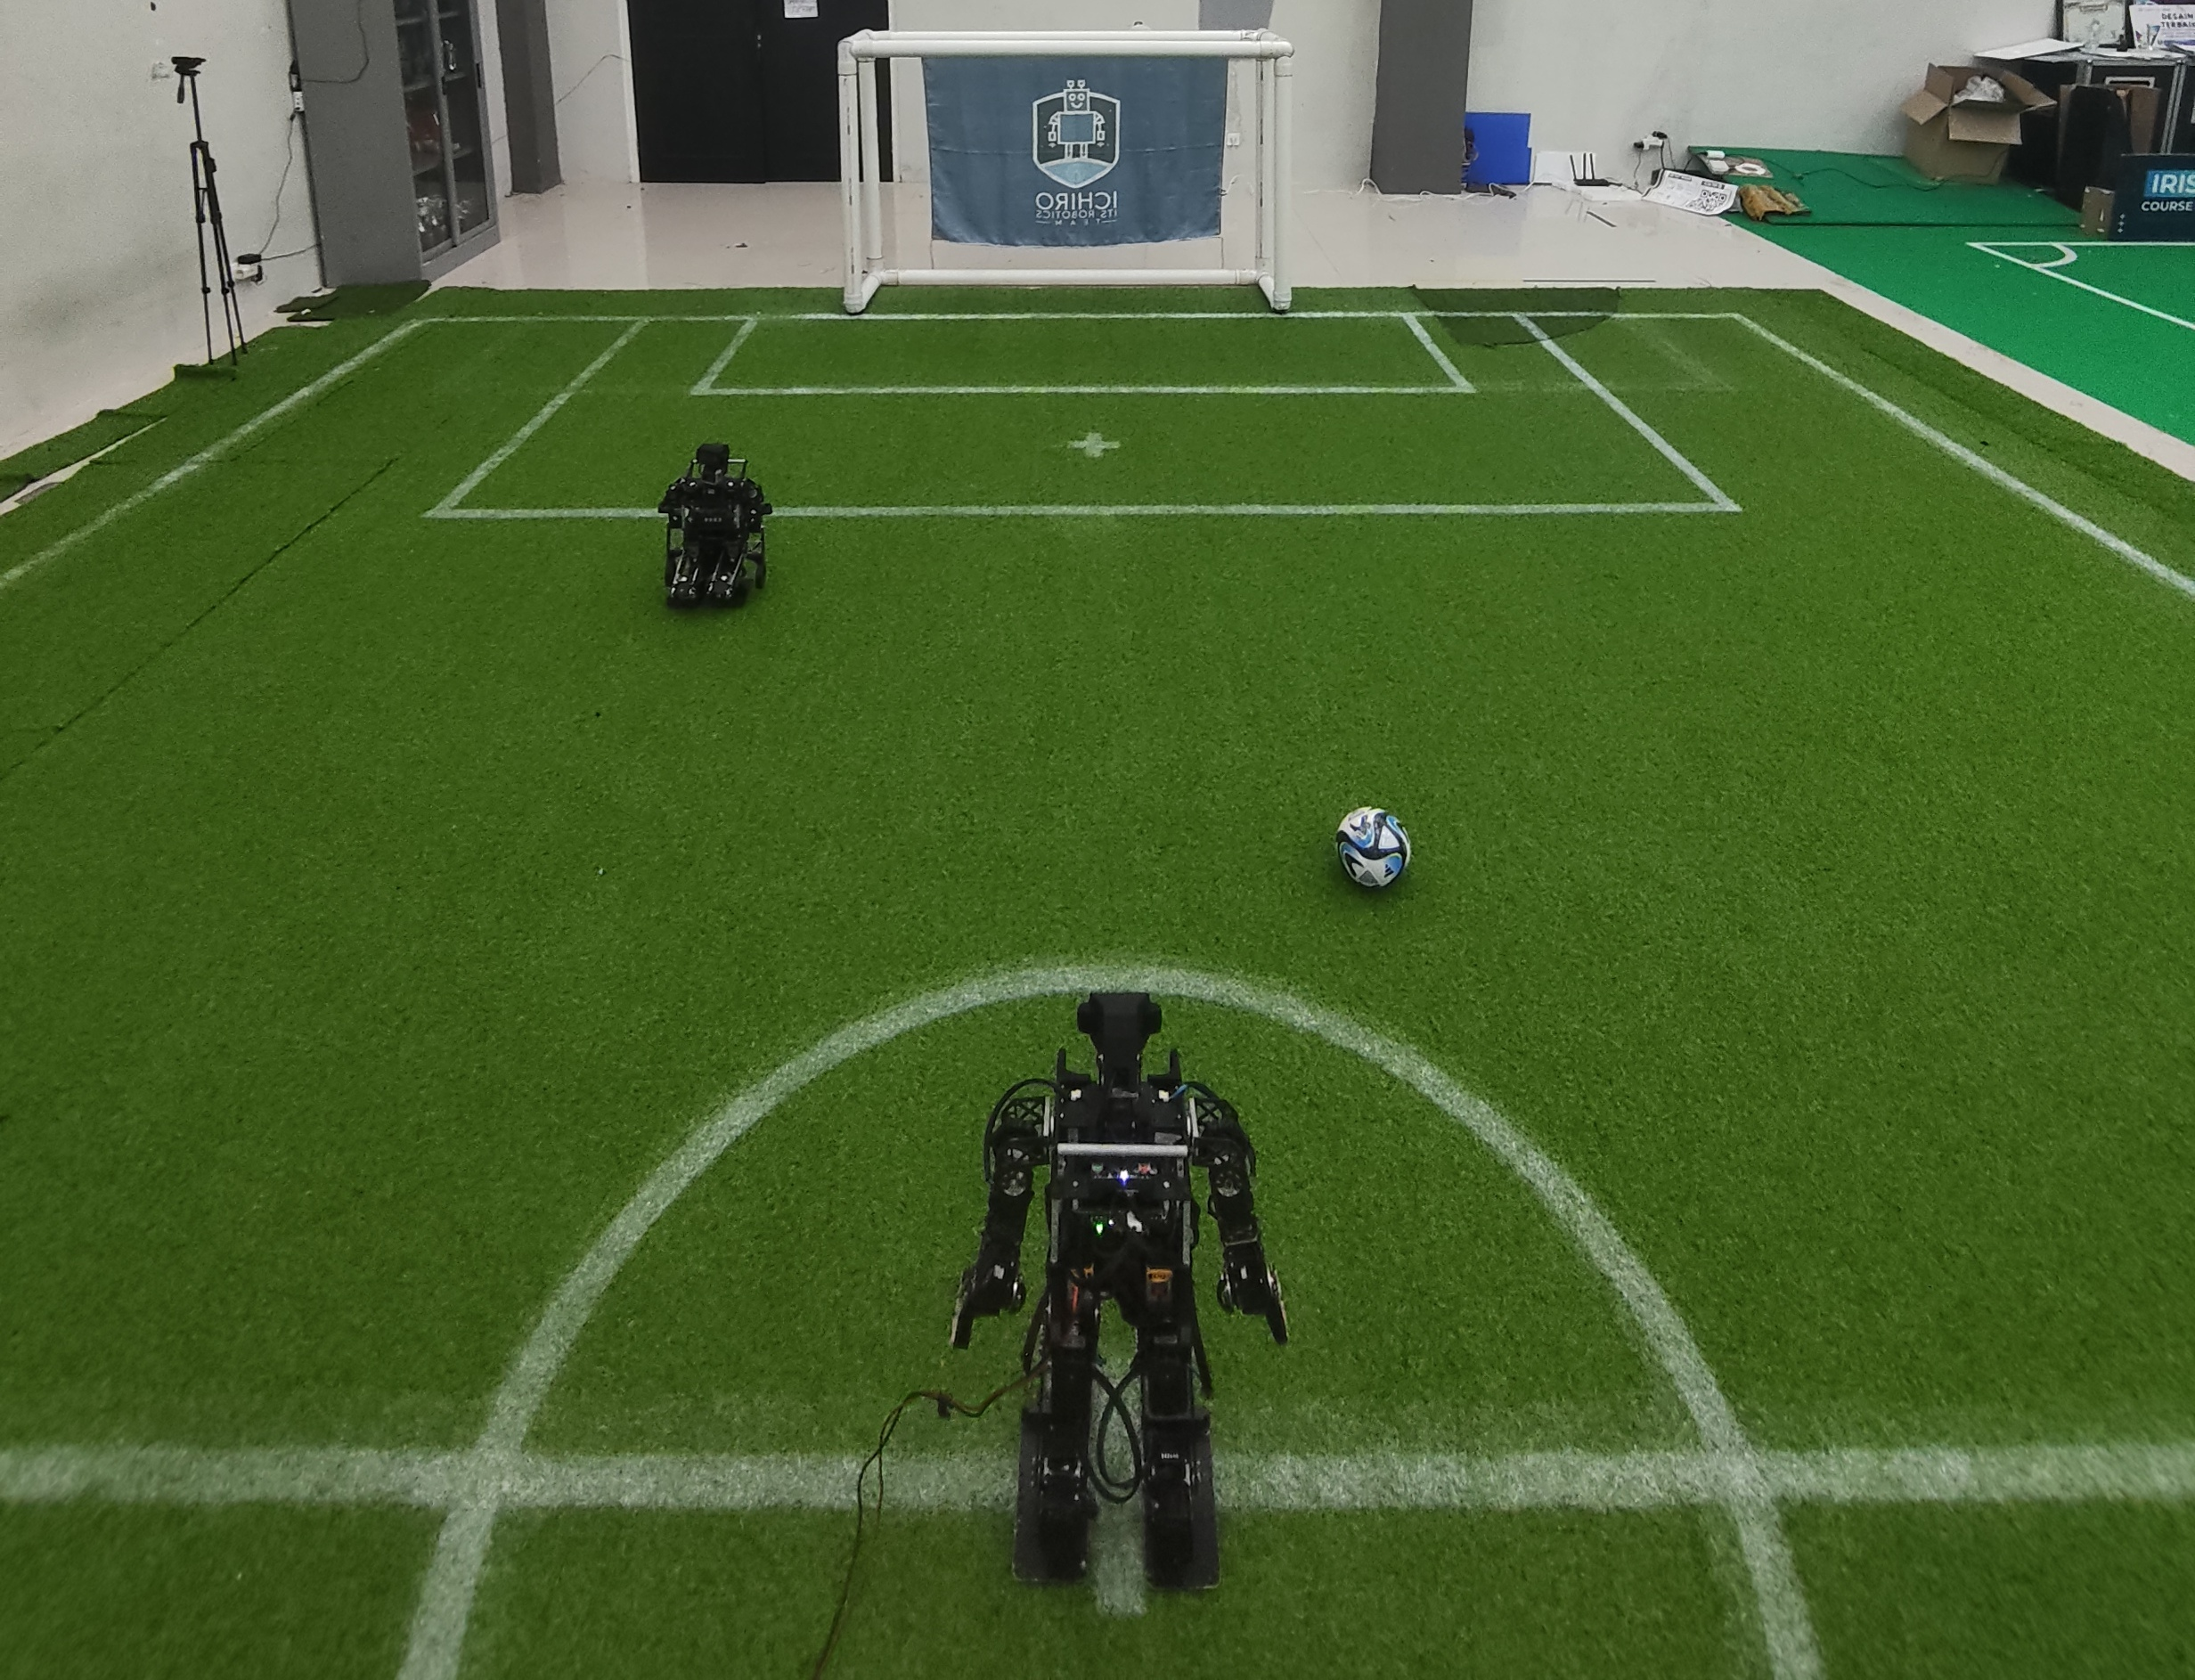
\includegraphics[width=0.5\textwidth]{Real Setup.jpg}
\caption{Actual experimental setup on the RoboCup field, showing the 
robot placement and physical arrangement of objects used during evaluation.}
\label{fig:real_setup}
\end{figure}

To assess the accuracy of the IPM estimations, three primary error metrics 
are defined for each observed object: the Euclidean error ($E$), the X-axis 
error ($E_x$), and the Y-axis error ($E_y$). These errors represents the overall 
geometric deviation between the estimated position $(\hat{X}, \hat{Y})$ and the ground-truth position 
$(X, Y)$, defined as:

\begin{equation}
E_x = \hat{X} - X, \quad
E_y = \hat{Y} - Y, \quad
E = \sqrt{(E_x )^2 + ( E_y )^2}
\end{equation}

To provide a normalized measure of error, the Euclidean error is expressed 
as a percentage relative to the distance between the robot's initial position 
$P(450.0, 300.0)$ and the object:

\begin{equation}
D = \sqrt{(X - X_0)^2 + (Y - Y_0)^2}
\end{equation}

\begin{equation}
E^{\%} = \frac{E}{D} \times 100\%
\end{equation}
Similarly, the axis-wise percentage errors are defined as:

\begin{equation}
E_x^{\%} = \frac{|E_x|}{|X - X_0|} \times 100\%, \quad
E_y^{\%} = \frac{|E_y|}{|Y - Y_0|} \times 100\%
\end{equation}


\subsection{Static Evaluation}

In static evaluation, the robot remains stationary at the kickoff 
position $P(450.0, 300.0)$, and both the body and head are kept fixed. 
Since the robot pose is known and does not change, it is treated 
as ground truth.

For each object, the IPM module estimates the relative position 
$(X_r, Y_r)$ with respect to the \texttt{base\_footprint} frame. 
The estimated global position $(\hat{X}_i, \hat{Y}_i)$ is obtained 
by applying a rigid body transformation using the known robot pose:

\begin{equation}
\begin{bmatrix}
\hat{X}_i \\
\hat{Y}_i \\
1
\end{bmatrix}
=
\mathbf{T}_{r}^{g}
\begin{bmatrix}
X_r \\
Y_r \\
1
\end{bmatrix}
\end{equation}

where $\mathbf{T}_{r}^{g}$ denotes the homogeneous transformation 
from the \texttt{base\_footprint} frame to the global field frame.

Table~\ref{tab:static_results} summarizes the static evaluation results, 
including the estimated positions, Euclidean error, and axis-wise errors 
reported in both absolute and percentage forms.

\begin{table}[h]
\centering
\footnotesize
\caption{Static IPM estimation results}
\label{tab:static_results}
\begin{tabular}{c c c c c}
\toprule
\textbf{Obj} & \textbf{$(\hat{X}, \hat{Y})$} & \textbf{$E$} & \textbf{$E_x$} & \textbf{$E_y$} \\
\midrule
$O_1$ & (548.1, 351.5) & 2.5 (2.2\%) & -1.9 (1.9\%) & 1.5 (3.1\%) \\
$O_2$ & (642.5, 200.5) & 7.5 (3.4\%) & -7.5 (3.8\%) & 0.5 (0.5\%) \\
$O_3$ & (752.3, 300.6) & 2.4 (0.8\%) & 2.3 (0.8\%) & 0.6 (0.0\%) \\
$O_4$ & (804.2, 443.6) & 7.7 (2.0\%) & 4.2 (1.2\%) & -6.4 (4.3\%) \\
$O_5$ & (930.1, 460.4) & 31.8 (6.7\%) & 30.1 (6.7\%) & 10.4 (6.9\%) \\
$O_6$ & (967.4, 168.7) & 67.4 (14.4\%) & 67.4 (15.0\%) & -1.3 (1.0\%) \\
\bottomrule
\end{tabular}
\end{table}

\subsection{Dynamic Evaluation}

The dynamic evaluation extends the experiment to conditions in 
which the robot is walking. The robot starts from the same kickoff 
position $P(450.0, 500.0)$ and walks forward for 1 meter toward target point 
$P'(550.0, 300.0)$, repeated for 10 trials.

During walking, the robot head performs continuous scanning motions 
to detect visible objects. The IPM module continuously estimates 
the relative object positions $(X_r, Y_r)$ in the 
\texttt{base\_footprint} frame.

To express object positions in global coordinates, the relative 
IPM outputs are transformed using the robot pose estimated from odometry:

\begin{equation}
\begin{bmatrix}
\hat{X}_i \\
\hat{Y}_i \\
1
\end{bmatrix}
=
\mathbf{T}_{r,\text{odom}}^{g}
\begin{bmatrix}
X_r \\
Y_r \\
1
\end{bmatrix}
\end{equation}

As in the static case, the error is computed as the Euclidean 
distance between the estimated and ground-truth object positions. 
In addition, axis-wise errors $(E_x, E_y)$ are reported to analyze 
directional bias.

Certain objects are excluded from the dynamic evaluation. In particular, 
the L-intersection ($O_4$) and T-intersection ($O_5$) are not considered, 
as multiple instances of these features are detected at different 
locations during walking. This ambiguity makes it difficult to associate 
detections with a unique ground-truth reference. Therefore, only objects 
with consistent and unambiguous detections are included in the analysis.

Table~\ref{tab:dynamic_results} presents the aggregated dynamic 
evaluation results.

\begin{table}[h]
\centering
\footnotesize
\caption{Dynamic IPM estimation results (aggregated over 10 trials)}
\label{tab:dynamic_results}
\begin{tabular}{c c c c}
\toprule
\textbf{Obj} & \textbf{Mean Estimated Position} & \textbf{$E$ (cm)} & \textbf{$(E_x, E_y)$ (cm)} \\
\midrule
$O_1$ & (551.7, 347.6) & 10.2 & (1.7, -2.4) \\
$O_2$ & (643.2, 203.2) & 19.0 & (-6.8, 3.2) \\
$O_3$ & (744.2, 299.9) & 11.2 & (-5.8, -0.1) \\
$O_6$ & (953.1, 177.7) & 68.2 & (53.1, 7.6) \\
\bottomrule
\end{tabular}
\end{table}

It is important to note that odometry is not involved in the IPM 
distance computation itself. IPM estimates object positions purely 
relative to the robot. Odometry is only used to express estimated 
object positions in global coordinates during dynamic evaluation. 
Therefore, the measured dynamic error is influenced by both IPM 
estimation error and odometry drift. To better understand this 
influence, odometry error is analyzed independently using the 
approach proposed by Martinelli~\cite{Martinelli2001APS}.

This method characterizes odometry uncertainty through four parameters: 
translational bias ($E_t$), translational noise ($K_\rho$), 
rotational bias ($E_r$), and rotational noise ($K_\theta$).
The parameters $E_t$ and $E_r$ represent \textit{systematic errors}, 
which correspond to consistent and repeatable deviations in robot motion, 
such as bias in traveled distance or heading. In contrast, the parameters 
$K_\rho$ and $K_\theta$ represent \textit{non-systematic errors}, which 
capture random variations caused by factors such as sensor noise and 
surface interaction.

The parameters are estimated by comparing the odometry-based pose 
$(x_{\text{odom}}, y_{\text{odom}}, \theta_{\text{odom}})$ with the 
ground-truth pose $(x_{\text{true}}, y_{\text{true}}, \theta_{\text{true}})$ 
over 10 trials of 1-meter forward motion. The resulting odometry 
error parameters are:
\begin{align*}
E_r &= -0.0005 \ \text{deg/cm}, \\
K_\theta &= 0.1995 \ \text{deg}^2/\text{cm}, \\
E_t &= -2.61\%, \\
K_\rho &= -0.0272 \ \text{cm}.
\end{align*}

The small magnitude of these parameters indicates that odometry error 
is limited and is unlikely to be the dominant source of error in the 
dynamic IPM results.

%\hfill mds
%\hfill January 11, 2007


% The contents of IAENG journals and proceedings books are
% peer-reviewed and archival. The journals and proceedings series
% publish scholarly articles of archival value as well as tutorial
% expositions and critical reviews of classical subjects and topics of
% current interest. Authors should consider the following points:

% 1) Technical papers submitted for publication must advance the state
% of knowledge and must cite relevant prior work.

% 2)  The length of a submitted paper should be commensurate with the
% importance, or appropriate to the complexity, of the work. For
% example, an obvious extension of previously published work might not
% be appropriate for publication or might be adequately treated in
% just a few pages.

% 3) Authors must convince both peer reviewers and the editors of the
% scientific and technical merit of a paper; the standards of proof
% are higher when extraordinary or unexpected results are reported.

% 4) Because replication is required for scientific progress, papers
% submitted for publication must provide sufficient information to
% allow readers to perform similar experiments or calculations and use
% the reported results. Although not everything need be disclosed, a
% paper must contain new, useable, and fully described information.
% For example, a specimen's chemical composition need not be reported
% if the main purpose of a paper is to introduce a new measurement
% technique. Authors should expect to be challenged by reviewers if
% the results are not supported by adequate data and critical details.

% 5)  Papers that describe ongoing work or announce the latest
% technical achievement, which are suitable for presentation at a
% professional conference, may not be appropriate for publication in a
% journal or proceedings book.

% Figure axis labels are often a source of confusion. Use words rather
% than symbols. As an example, write the quantity "Magnetization," or
% "Magnetization M," not just "M." Put units in parentheses. Do not
% label axes only with units.

% Large figures and tables may span both columns. Place figure
% captions below the figures; place table titles above the tables. If
% your figure has two parts, include the labels "(a)" and "(b)" as
% part of the artwork. Please verify that the figures and tables you
% mention in the text actually exist.


% Note that IAENG typically puts floats only at the top, even when this
% results in a large percentage of a column being occupied by floats.


% An example of a double column floating figure using two subfigures.
% (The subfig.sty package must be loaded for this to work.)
% The subfigure \label commands are set within each subfloat command, the
% \label for the overall figure must come after \caption.
% \hfil must be used as a separator to get equal spacing.
% The subfigure.sty package works much the same way, except \subfigure is
% used instead of \subfloat.
%
%\begin{figure*}[!t]
%\centerline{\subfloat[Case I]\includegraphics[width=2.5in]{subfigcase1}%
%\label{fig_first_case}}
%\hfil
%\subfloat[Case II]{\includegraphics[width=2.5in]{subfigcase2}%
%\label{fig_second_case}}}
%\caption{Simulation results}
%\label{fig_sim}
%\end{figure*}
%
% Note that often IAENG papers with subfigures do not employ subfigure
% captions (using the optional argument to \subfloat), but instead will
% reference/describe all of them (a), (b), etc., within the main caption.


% An example of a floating table. Note that, for IAENG style tables, the
% \caption command should come BEFORE the table. Table text will default to
% \footnotesize as IAENG normally uses this smaller font for tables.
% The \label must come after \caption as always.
%
%\begin{table}[!t]
%% increase table row spacing, adjust to taste
%\renewcommand{\arraystretch}{1.3}
% if using array.sty, it might be a good idea to tweak the value of
% \extrarowheight as needed to properly center the text within the cells
%\caption{An Example of a Table}
%\label{table_example}
%\centering
%% Some packages, such as MDW tools, offer better commands for making tables
%% than the plain LaTeX2e tabular which is used here.
%\begin{tabular}{|c||c||c|}
%\hline
%One & Two & Five\\
%\hline
%Two & Four & Ten\\
%\hline
%\end{tabular}
%\end{table}


% Note that IAENG does not put floats in the very first column - or typically
% anywhere on the first page for that matter. Also, in-text middle ("here")
% positioning is not used. Most IAENG journals use top floats exclusively.
% Note that, LaTeX2e, unlike IAENG journals, places footnotes above bottom
% floats. This can be corrected via the \fnbelowfloat command of the
% stfloats package.


\section{Conclusion}
The conclusion goes here. what

A conclusion section is not compulsory. Although a conclusion may
review the main points of the paper, do not replicate the abstract
as the conclusion. A conclusion might elaborate on the importance of
the work or suggest applications and extensions.


% Can use something like this to put references on a page
% by themselves when using endfloat and the captionsoff option.
% \ifCLASSOPTIONcaptionsoff
%   \newpage
% \fi



% trigger a \newpage just before the given reference
% number - used to balance the columns on the last page
% adjust value as needed - may need to be readjusted if
% the document is modified later
%\IAENGtriggeratref{8}
% The "triggered" command can be changed if desired:
%\IAENGtriggercmd{\enlargethispage{-5in}}

% references section

% can use a bibliography generated by BibTeX as a .bbl file
% BibTeX documentation can be easily obtained at:
% http://www.ctan.org/tex-archive/biblio/bibtex/contrib/doc/
% The IAENGtran BibTeX style support page is at:
% http://www.michaelshell.org/tex/IAENGtran/bibtex/
%\bibliographystyle{IAENGtran}
% argument is your BibTeX string definitions and bibliography database(s)
%\bibliography{IAENGabrv,../bib/paper}
%
% <OR> manually copy in the resultant .bbl file
% set second argument of \begin to the number of references
% (used to reserve space for the reference number labels box)
% \begin{thebibliography}{1}

% \bibitem{IJCS}
% N.~Meghanathan and G.~W. Skelton, ``Risk Notification Message
% Dissemination Protocol for Energy Efficient Broadcast in Vehicular
% Ad hoc Networks,'' {\it IAENG International Journal of Computer
% Science}, vol. 37, no. 1, pp. 1-10, Jul. 2010.

% \end{thebibliography}


% >>>>>>>>>>>>>>>>>>>>>> Bibliography <<<<<<<<<<<<<<<<<<<<<<<<<<<<<<<<<<<<<

\bibliographystyle{BibTeXtran}   % (uses file "BibTeXtran.bst")
\bibliography{BibTeXrefs}       % (expects the reference in the file "BibTeXrefs.bib")

\end{document}
